\documentclass[10pt, xetex, handout]{beamer}

\usetheme[
    progressbar=frametitle, 
    block=fill
]{metropolis}
\usepackage{appendixnumberbeamer}

\usefonttheme[onlymath]{serif}

\usepackage[italian]{babel}
\usepackage{booktabs}
\usepackage[scale=2]{ccicons}
\usepackage{float}

\usepackage{tikz}
\usetikzlibrary{calc}
\usetikzlibrary{quotes}
\usetikzlibrary{patterns}
\usetikzlibrary{angles}
% \usetikzlibrary{external}
% \tikzexternalize[prefix=tikz/]

\usepackage[european]{circuitikz}
\usepackage{tikz-timing}
\usepackage{tikzscale}

\usepackage{pgfplots}
\usepgfplotslibrary{dateplot}

\usepackage{xspace}

% maths
\usepackage{amsmath}
\usepackage{amssymb}
\usepackage{amsthm}
\newcommand{\dd}[1]{\mathrm{d}#1}


\title{Spectrum Analyzer}
\subtitle{Lavoro Professionale Individuale}
\date{\today}
\author{Naoki Pross}
\institute{SAM Bellinzona}
\titlegraphic{\hfill
\includegraphics[height=1.3cm]{figures/logo/LOGO_SAM.pdf}}

\begin{document}

\maketitle

\begin{frame}{Table of contents}
    \setbeamertemplate{section in toc}[sections numbered]
    \tableofcontents[hideallsubsections]
\end{frame}

\section{Introduzione}
\begin{frame}{A cosa servono l'analisi spettrale e la FT?}
    \vfill
    Alcuni esempi pratici
    \begin{description}
        \item [Elettronica] Filtri digitali, analisi di segnali
        \item [Informatica] Audio editing, Riconoscimento sonoro / vocale
        \item [Matematica] Risoluzione di equazioni differenziali
        \item [Fisica] Principio di inteterminazione di Heisenberg
    \end{description}
    \vfill
    \begin{figure} \centering
        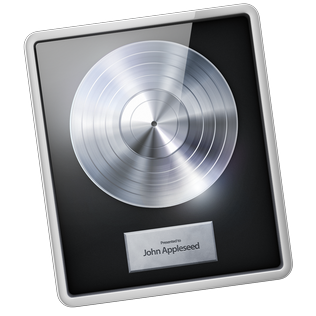
\includegraphics[height=1.5cm]{figures/logo/logic}
        \hfill
        
\includegraphics[height=1.5cm]{figures/logo/shazam}
        \hfill
        
\includegraphics[height=1.5cm]{figures/logo/siri}
        \hfill
        \begin{minipage}[b][1.5cm][c]{.25\linewidth}
        \begin{align*}
            \langle x\,|\,\hat p\,|\,\psi \rangle &= 
                -i\mathbf{\hbar}\frac{d}{dx} \psi(x) \\
            \langle x\,|\,\hat x\,|\,\psi \rangle &= 
                i\mathbf{\hbar}\frac{d}{dp} \psi(p) \\
        \end{align*}
        \end{minipage}
    \end{figure}
\end{frame}

\begin{frame}{Obiettivo}
    Realizzare un circuito di analisi spettrale
    \begin{block}{Requisiti}
    \begin{itemize}
        \item Analisi dello spettro fino a 10\,kHz
        \item Entrate Jack e RCA
        \item Visualizzazione 
        \item Utilizzo di un PIC18F45K22
    \end{itemize}
    \end{block}
    
    \pause
    \begin{block}{Componenti}
    \begin{itemize}
        \item Circuito di adattamento in entrata
        \item Design di un PCB
        \item Software per il uC e per il PC
    \end{itemize}
    \end{block}
\end{frame}

\begin{frame}{Schema a blocchi}
    \begin{figure} \centering
    \resizebox{\textwidth}{!}{
        \includegraphics{figures/block-diagram.tikz}
    }
    \end{figure}
\end{frame}

\section{Fourier Transform}
\begin{frame}{Rappresentazione grafica}
    \begin{figure} \centering
        \includegraphics{figures/fourier-3d-plot.tikz}
    \end{figure}
    \[
        \hat{f\,} (\omega) 
        = \int_{-\infty}^\infty f\,(x)\,\cdot e^{-i\omega x}\,\dd{x}
    \]
\end{frame}

\section{Fast Fourier Transform}
\begin{frame}{Divide et impera (Divide and Conquer)}
    La FFT appartiene ad una classe di algoritmi chiamata
    \begin{center}
        \Large Divide et Impera
    \end{center}

    \begin{block}{Definizione}
    \begin{enumerate}
        \item \emph{Divide} il problema in sottoproblemi
        \item \emph{Impera} (conquista) i sottoproblemi
        \item \emph{Combina} i risultati dei sottoproblemi
    \end{enumerate}
    \end{block}
\end{frame}

\begin{frame}{Il problema della DFT}
    La trasformata di Fourier discreta \`e
    \[
        \vec{X} = \mathbf{V}\cdot\vec{x}_n
    \]
    In cui
    \[
        \mathbf{V} = 
        \begin{pmatrix}
        1      & 1                      & 1                       & \dots  & 1                        \\[1em]
        1      & (e^{i\omega})^{-1}     & (e^{i\omega})^{-2}      & \dots  & (e^{i\omega})^{-(N-1)}   \\[1em]
        1      & (e^{i\omega})^{-2}     & (e^{i\omega})^{-4}      & \dots  & (e^{i\omega})^{-2(N-1)}  \\[1em]
        \vdots & \vdots                 &  \vdots                 & \ddots & \vdots                   \\[1em]
        1      & (e^{i\omega})^{-(N-1)} & (e^{i\omega})^{-2(N-1)} & \dots  & (e^{i\omega})^{-(N-1)^2} \\[1em]
        \end{pmatrix}
    \]
\end{frame}

\begin{frame}{Complessit\`a temporale (analisi asintotica)}
    \begin{block}{Definizione}
        In informatica, la complessità temporale di un algoritmo quantifica la
        quantità di tempo impiegata da un algoritmo a essere eseguito.
    \end{block}
    Descrivendo il prodotto nelle componenti
    \[
        X_k = \sum_{n=0}^{N-1} x_n\cdot e^{-i\omega kn}
        \qquad 0 \leq k < N
    \]
    Osserviamo che la complessit\`a temporale \`e \(\mathcal{O}(N^2)\).
\end{frame}


\section{Prodotto realizzato}
\begin{frame}{Hardware Analogico}
    \begin{figure}
        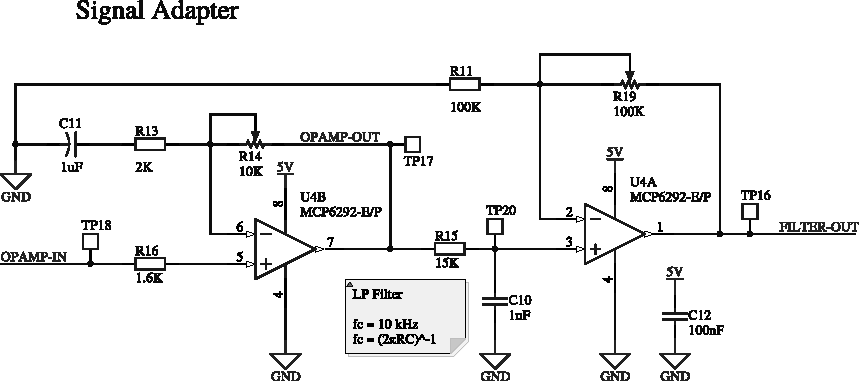
\includegraphics[width=\linewidth]{figures/circuits/filter-ampl-v2}
    \end{figure}
\end{frame}

\begin{frame}{FFT Software}
    L'implementazione si chiama
    \vfill
    \begin{center}
        \Large Fixed-Point In-Place FFT
    \end{center}
    \vfill
    \begin{description}
        \item [Fixed-Point] Il numero di bit per la mantissa e per
            l'esponente del valore floating point sono costanti
        \item [In-Place] I risultati sovrascrivono i dati di partenza
        \item [FFT] Fast Fourier Transform
    \end{description}
\end{frame}

\begin{frame}{Software}
    \begin{center}
        \Large Demo!
    \end{center}
\end{frame}

\section{Conclusioni}
\begin{frame}{Obiettivi}
    \begin{block}{Raggiungi}
    \begin{itemize}
        \item Analisi spettrale fino a 10\,kHz
        \item Visualizzazione al PC\(^\dagger\)
        \item Esportare immagini / dati
    \end{itemize}
    \end{block}
    \pause

    \begin{block}{Incompleti}
    \begin{itemize}
        \item \(^\dagger\) Visualizzazione delle curve \(\Re(z)\) e \(\Im(z)\) in un solo grafico
        \item Visualizzazione mediante la matrice LED
    \end{itemize}
    \end{block}
\end{frame}

\begin{frame}{Possibili miglioramenti}
\end{frame}


\end{document}
